\documentclass[dvipdfmx,cjk,xcolor=dvipsnames,envcountsect,notheorems,12pt]{beamer}
% * 16:9 のスライドを作るときは、aspectratio=169 を documentclass のオプションに追加する
% * 印刷用の配布資料を作るときは handout を documentclass のオプションに追加する
%   (overlay が全て一つのスライドに出力される)

\usepackage{pxjahyper}% しおりの文字化け対策 (なくても良い)
\usepackage{amsmath,amssymb,amsfonts,amsthm,ascmac,cases,bm,pifont}
\usepackage{graphicx}
\usepackage{bussproofs}
\usepackage{url}
\usepackage{etex}

% スライドのテーマ
\usetheme{sumiilab}
% ベースになる色を指定できる
%\usecolortheme[named=Magenta]{structure}
% 数式の文字が細くて見難い時は serif の代わりに bold にしましょう
%\mathversion{bold}

%% ===============================================
%% スライドの表紙および PDF に表示される情報
%% ===============================================

%% 発表会の名前とか(省略可)
\session{平成27年度 卒業研究発表会}
%% スライドのタイトル
\title{MinCamlのK正規化の形式的検証}
%% 必要ならば、サブタイトルも
%\subtitle{}
%% 発表者のお名前
\author{B2TB2512 水野雅之}
%% 発表者の所属([] 内は短い名前)
\institute[東北大学 住井・松田研]{工学部 情報知能システム総合学科\\住井・松田研究室}% 学部生
%\institute[東北大学 住井・松田研]{大学院情報科学研究科 情報基礎科学専攻\\住井・松田研究室}% 院生
%% 発表する日
\date{2016年3月11日}

%% ===============================================
%% 自動挿入される目次ページの設定(削除しても可)
%% ===============================================

%% section の先頭に自動挿入される目次ページ(削除すると、表示されなくなる)
\AtBeginSection[]{
\begin{frame}
  \frametitle{アウトライン}
  \tableofcontents[sectionstyle=show/shaded,subsectionstyle=show/show/hide]
\end{frame}}
%% subsection の先頭に自動挿入される目次ページ(削除すると、表示されなくなる)
\AtBeginSubsection[]{
\begin{frame}
  \frametitle{アウトライン}
  \tableofcontents[sectionstyle=show/shaded,subsectionstyle=show/shaded/hide]
\end{frame}}

%% 現在の section 以外を非表示にする場合は以下のようにする

%% \AtBeginSection[]{
%% \begin{frame}
%%   \frametitle{アウトライン}
%%   \tableofcontents[sectionstyle=show/hide,subsectionstyle=show/show/hide]
%% \end{frame}}
%% \AtBeginSubsection[]{
%% \begin{frame}
%%   \frametitle{アウトライン}
%%   \tableofcontents[sectionstyle=show/hide,subsectionstyle=show/shaded/hide]
%% \end{frame}}

%% ===============================================
%% 定理環境の設定
%% ===============================================

\setbeamertemplate{theorems}[numbered]% 定理環境に番号を付ける
\theoremstyle{definition}
\newtheorem{definition}{定義}
\newtheorem{axiom}{公理}
\newtheorem{theorem}{定理}
\newtheorem{lemma}{補題}
\newtheorem{corollary}{系}
\newtheorem{proposition}{命題}

%% ===============================================
%% ソースコードの設定
%% ===============================================

\usepackage{listings,jlisting}
%\usepackage[scale=0.9]{DejaVuSansMono}

\definecolor{DarkGreen}{rgb}{0,0.5,0}
% プログラミング言語と表示するフォント等の設定
\lstset{
  language={[Objective]Caml},% プログラミング言語
  basicstyle={\ttfamily\small},% ソースコードのテキストのスタイル
  keywordstyle={\bfseries},% 予約語等のキーワードのスタイル
  commentstyle={},% コメントのスタイル
  stringstyle={},% 文字列のスタイル
  frame=trlb,% ソースコードの枠線の設定 (none だと非表示)
  numbers=none,% 行番号の表示 (left だと左に表示)
  numberstyle={},% 行番号のスタイル
  xleftmargin=5pt,% 左余白
  xrightmargin=5pt,% 右余白
  keepspaces=true,% 空白を表示する
  mathescape,% $ で囲った部分を数式として表示する ($ がソースコード中で使えなくなるので注意)
  % 手動強調表示の設定
  moredelim=[is][\itshape]{@/}{/@},
  moredelim=[is][\color{red}]{@r\{}{\}@},
  moredelim=[is][\color{blue}]{@b\{}{\}@},
  moredelim=[is][\color{DarkGreen}]{@g\{}{\}@},
}

\newcommand{\keyword}[1]{\mathbf{#1}}
\newcommand{\LET}{\keyword{let}}
\newcommand{\REC}{\keyword{rec}}
\newcommand{\ARRAY}{\keyword{Array}}
\newcommand{\CREATE}{\keyword{create}}
\newcommand{\AND}{\keyword{and}}
\newcommand{\IN}{\keyword{in}}
\newcommand{\TRUE}{\keyword{true}}
\newcommand{\WHILE}{\keyword{while}}
\newcommand{\DO}{\keyword{do}}
\newcommand{\DONE}{\keyword{done}}

%% ===============================================
%% 本文
%% ===============================================
\begin{document}
\frame[plain]{\titlepage}% タイトルページ

\begin{frame}
	\frametitle{研究目的}
	\LARGE MinCamlの正当性を形式的に検証
	\begin{itemize}
		\item 証明を簡潔に
			\begin{itemize}
				\item de Buijnインデックス
				\item 余帰納的大ステップ意味論
			\end{itemize}
		\item スケーラビリティの確保
			\begin{itemize}
				\item 証明自動化機能を活用
			\end{itemize}
	\end{itemize}
\end{frame}

\section*{アウトライン}

% 目次を表示させる(section を表示し、subsection は隠す)
\begin{frame}
  \frametitle{アウトライン}
  \tableofcontents[sectionstyle=show,subsectionstyle=hide]
\end{frame}

\section{研究背景}

\begin{frame}
	\frametitle{コンパイラの形式的検証の意義}
	\LARGE コンパイラのバグ
	\begin{itemize}
		\item 広範囲に影響が及ぶ
		\item デバッグが困難
	\end{itemize}
\end{frame}

\begin{frame}
	\frametitle{関連研究}
	\LARGE CompCert [Leroyら 2006]
	\begin{itemize}
		\item Cコンパイラの正当性の検証
	\end{itemize}

	[Chlipala 2010]
	\begin{itemize}
		\item 非純粋関数型言語処理系の正当性の検証
	\end{itemize}
\end{frame}

\begin{frame}
	\frametitle{本研究の目標と現状}
	\Large 目標:MinCamlの正当性を検証

	\vfill

	現状:サブセットのK正規化の正当性を検証
	\begin{center}
		\normalsize
		\begin{tabular}{ll}
			実装済 & 1引数関数、算術演算、let、if \\
			未実装 & タプル、複数引数関数、配列、外部関数呼び出し \\
		\end{tabular}
	\end{center}
\end{frame}

\section{MinCaml}

\begin{frame}
	\frametitle{MinCamlの特徴}
	\Large 住井による教育用コンパイラ [FDPE 2005]
	\begin{itemize}
		\item 非純粋な関数型言語
		\item OCamlで2000行程度の実装
			\begin{itemize}
				\item 型推論
				\item 定数畳み込み等の最適化
			\end{itemize}
	\end{itemize}
\end{frame}

\begin{frame}
	\frametitle{対象言語}
	\Large
	\begin{itemize}
		\item \alert<1>{高階関数}
		\item \alert<2>{N引数の構文}
		\item \alert<3>{副作用}
		\item \alert<4>{外部関数呼び出し(入出力)}
	\end{itemize}
	{\normalsize
	\[
	\begin{array}{l}
		M, N ::= \\
		\qquad \qquad \vdots\\
		\qquad \alert<1>{\LET~\REC~x~y_1~\cdots~y_n=M~\IN~N}\\
		\qquad \alert<1,2,4>{M~N_1~\cdots~N_n}\\
		\qquad \alert<2>{(M_1,~\cdots~,M_n)}\\
		\qquad \LET~(x_1,~\cdots~,x_n)=M~\IN~N\\
		\qquad \alert<3>{\ARRAY.\CREATE~M~N}\\
		\qquad \alert<3>{M_1.(M_2)}\\
		\qquad \alert<3>{M_1.(M_2)\leftarrow M_3}\\
	\end{array}
	\]}
	\pause
	\pause
	\pause
\end{frame}

\begin{frame}
	\frametitle{内部設計}
	\begin{itemize}
		\item 様々なコンパイルフェーズ
		\item 疎結合
	\end{itemize}

	\begin{figure}[htb]
		\centering
		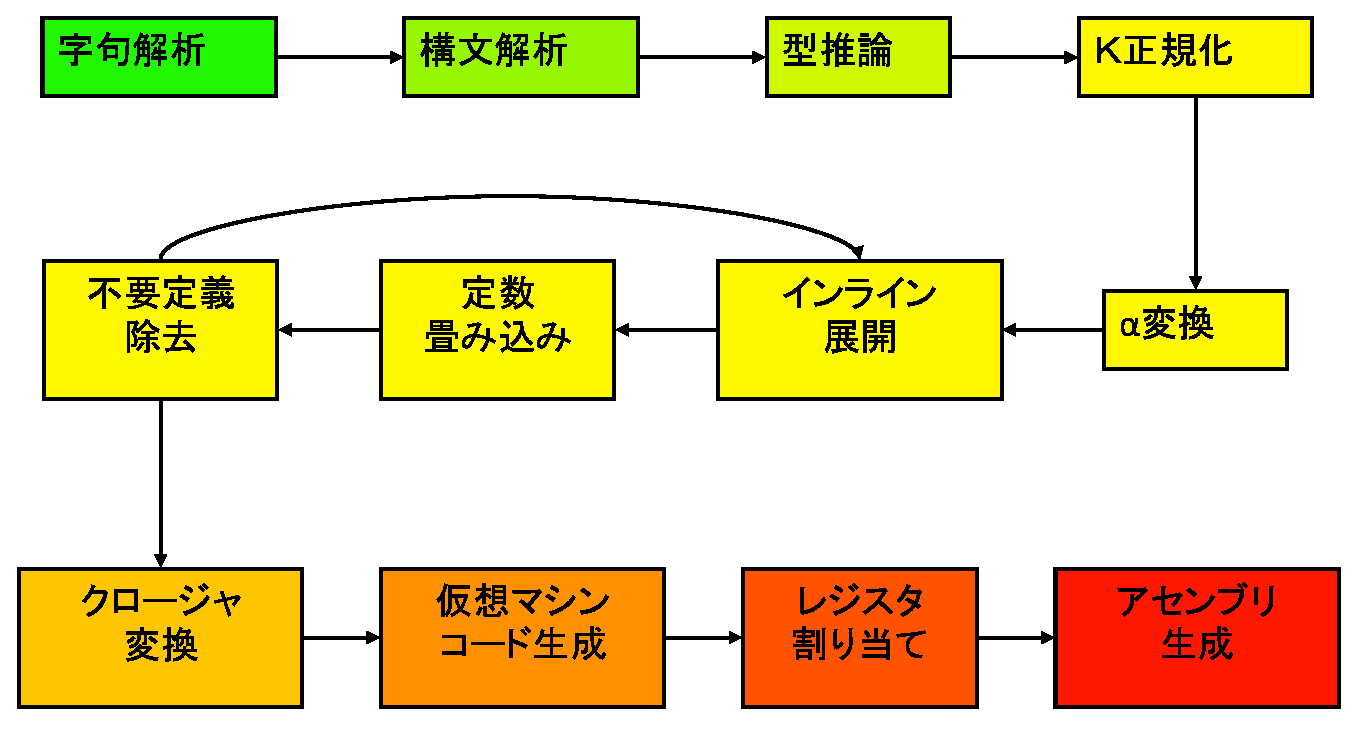
\includegraphics[width=8cm,clip]{mincaml.eps}
	\end{figure}
	{\footnotesize \url{http://esumii.github.io/min-caml/index8.html}}
\end{frame}

\begin{frame}
	\frametitle{K正規化}
	\LARGE
	全ての部分式に名前を付ける

	\begin{columns}
		\begin{column}{0.5\textwidth}
			\begin{center}
				$a+b*c+d$
			\end{center}
		\end{column}
		\begin{column}{0.5\textwidth}
			\begin{center}
				\[
					\begin{array}{l}
						\alert<2>{\LET~x =} b * c~\alert<2>{\IN} \\
						\alert<2>{\LET~y =} a + x~\alert<2>{\IN} \\
						y + d
					\end{array}
				\]
			\end{center}
		\end{column}
	\end{columns}

	\vfill

	\alert<2>{束縛に関する操作}
	\pause
\end{frame}

\begin{frame}
	\frametitle{期待される定理(1/2)}
	{\LARGE K正規化後の項を評価してみる}

	\vfill

	\Large 単純な値では一致
	{\normalsize \begin{columns}
		\begin{column}{0.4\textwidth}
			\[ 1+2\Downarrow 3 \]
		\end{column}
		\begin{column}{0.4\textwidth}
			\[ 
				\begin{array}{l}
					\LET~a = 1~\IN \\
					\LET~b = 2~\IN \\
					a + b\Downarrow 3
				\end{array}
			\]
		\end{column}
	\end{columns}}

	\vfill

	元の値のK正規形と一致
	{\normalsize \begin{columns}
		\begin{column}{0.4\textwidth}
			\[
				\begin{array}{l}
					\lambda x.\lambda y.\lambda z.~x+y+z\\
					\Downarrow \lambda x.\lambda y.\lambda z.~x+y+z
				\end{array}
			\]
		\end{column}
		\begin{column}{0.4\textwidth}
			\[ 
				\begin{array}{l}
					\lambda x.\lambda y.\lambda z.\\
					\LET~a = x+y~\IN \\
					a + z \\
					\Downarrow \lambda x.\lambda y.\lambda z.\\
					\LET~a = x+y~\IN \\
					a + z \\
				\end{array}
			\]
		\end{column}
	\end{columns}}
\end{frame}

\begin{frame}
	\frametitle{期待される定理(2/2)}
	{\Large
	\begin{theorem}
		項tが値vに評価される場合、項tをK正規化した結果K(t)は値vをK正規化した結果K(v)に評価される
	\end{theorem}
	\begin{theorem}
		項tの評価が停止しない場合、項tをK正規化した結果K(t)の評価は停止しない
	\end{theorem}}
	\Large 今回検証した言語の範囲では評価は決定的なため、逆も成り立つ

\end{frame}

\section{束縛の表現}

\begin{frame}
	\frametitle{名前による表現の問題点}
	\LARGE $\alpha$等価性の議論が面倒
	\[ \lambda x.\lambda y.~x \simeq \lambda a.\lambda b.~a \]

	\vfill

	freshな名前が必要になる
	\begin{itemize}
		\item 束縛の関係を乱さないよう変数名を選ぶ
	\end{itemize}
	\[
		\begin{array}{lcl}
			[x \mapsto z](\lambda z.~x) & \simeq & \lambda z'.~z \\
																	& \not \simeq & \lambda z.~z
		\end{array}
	\]
\end{frame}

\begin{frame}
	\frametitle{de Buijnインデックス}
	\LARGE
	何番目の束縛かで変数を表現
	\begin{itemize}
		\item 内側から外側へ数える
	\end{itemize}
	\begin{columns}
		\begin{column}{0.5\textwidth}
			\[ \lambda x. \lambda y. \lambda z.~x z (y z) \]
		\end{column}
		\begin{column}{0.5\textwidth}
			\[ \lambda. \lambda. \lambda.~2~0~(1~0) \]
		\end{column}
	\end{columns}

	\vfill

	$\alpha$等価な式は構文的に等価
	\begin{itemize}
		\item 名前のfreshnessを保証
	\end{itemize}
	\begin{columns}
		\begin{column}{0.5\textwidth}
			\[ \lambda x.\lambda y.~x \]
			\[ \lambda a.\lambda b.~a \]
		\end{column}
		\begin{column}{0.5\textwidth}
			\[ \lambda.\lambda.~1 \]
		\end{column}
	\end{columns}
\end{frame}

\begin{frame}
	\frametitle{シフト}
	\LARGE 自由変数のインデックスをずらす
	\[\uparrow^d t \]

	束縛に関する操作
	{\large \begin{columns}
		\begin{column}{0.5\textwidth}
			\[ (\lambda x.~x)~(\lambda y.~z) \]
		\end{column}
		\begin{column}{0.5\textwidth}
			\[ (\lambda.~0)~\alert{(\lambda.~1)} \]
		\end{column}
	\end{columns}

	\vfill

	\begin{columns}
		\begin{column}{0.5\textwidth}
			\[ 
					\begin{array}{l}
						\LET~a = \lambda x.~x~\IN \\
						\LET~b = \lambda y.~z~\IN \\
						a~b
					\end{array}
			\]
		\end{column}
		\begin{column}{0.5\textwidth}
			\[
				\begin{array}{l}
					\LET~\_ = \lambda.~0~\IN \\
					\LET~\_ = \alert{\only<1>{\uparrow^1(\lambda.~1)}\only<2->{\lambda.~2}}~\IN \\
					1~0
				\end{array}
			\]
		\end{column}
	\end{columns}}
	\pause
\end{frame}

\begin{frame}[fragile]
	\frametitle{K正規化の実装}
\begin{lstlisting}[basicstyle={\ttfamily\normalsize}]
Fixpoint knormal e :=
  match e with
  | Exp.Var x => K.Var x
  | Exp.Abs e => K.Abs (knormal e)
  | Exp.App e1 e2 =>
      K.Let (knormal e1)
        (K.Let (shift 1 (knormal e2))
          (App 1 0))
  end.
\end{lstlisting}
\end{frame}

\section{意味論の定義}

\begin{frame}
	\frametitle{大ステップ意味論}
	\LARGE
	\begin{center}
	比較的単純な\\プログラム変換の検証に適する

	\vfill

	が

	\vfill

	無限ループとエラーの区別が困難
	\end{center}
\end{frame}

\begin{frame}
	\frametitle{例:型無しラムダ計算}
	\Large
	構文
	\begin{columns}
		\begin{column}{0.5\textwidth}
			\[
				\begin{array}{lcl}
					t & ::= & b \\
					  & | & x \\
						& | & \lambda x.~t \\
						& | & t~t
				\end{array}
			\]
		\end{column}
		\begin{column}{0.5\textwidth}
			\[
				\begin{array}{lcl}
					v & ::= & b \\
						& | & \lambda x.~t \\
				\end{array}
			\]
		\end{column}
	\end{columns}

	\vfill

	意味論
	\begin{columns}
		\begin{column}{0.5\textwidth}
			\[\overline{b \Downarrow b}\]
		\end{column}
		\begin{column}{0.5\textwidth}
			\[\overline{\lambda x.~t \Downarrow \lambda x.~t}\]
		\end{column}
	\end{columns}

	\begin{prooftree}
		\AxiomC{$t_1 \Downarrow \lambda x.~t$}
		\AxiomC{$t_2 \Downarrow v_2$}
		\AxiomC{$[x \mapsto v_2]t \Downarrow v$}
		\TrinaryInfC{$t_1~t_2 \Downarrow v$}
	\end{prooftree}
\end{frame}

\begin{frame}
	\frametitle{大ステップ意味論の問題点}
	\begin{columns}
		\begin{column}{0.4\textwidth}
			{\LARGE エラー}
			{\Large \[ \TRUE~\TRUE \not \Downarrow v \]}
			適用できる規則が無い
		\end{column}
		\begin{column}{0.6\textwidth}
			{\LARGE 無限ループ}
			{\Large \[ ~(\lambda x.xx)(\lambda x.xx) \not \Downarrow v \]}
			有限回の規則適用で導出できない
		\end{column}
	\end{columns}

	\vfill

	\begin{center}
		{\LARGE 区別できない}
	\end{center}
\end{frame}

\begin{frame}
	\frametitle{余帰納的大ステップ意味論(1/2)}
	\LARGE
	余帰納的に定義 [Leroy, Grall 2009]
	\begin{columns}
		\begin{column}{0.3\textwidth}
			\begin{prooftree}
				\AxiomC{$t_1 \Uparrow$}
				\doubleLine
				\UnaryInfC{$t_1~t_2 \Uparrow$}
			\end{prooftree}
		\end{column}
		\begin{column}{0.7\textwidth}
			\begin{prooftree}
				\AxiomC{$t_1 \Downarrow v_1$}
				\AxiomC{$t_2 \Uparrow$}
				\doubleLine
				\BinaryInfC{$t_1~t_2 \Uparrow$}
			\end{prooftree}
		\end{column}
	\end{columns}

	\vfill

	\begin{prooftree}
		\AxiomC{$t_1 \Downarrow \lambda x.~t$}
		\AxiomC{$t_2 \Downarrow v_2$}
		\AxiomC{$[x \mapsto v_2]t \Uparrow$}
		\doubleLine
		\TrinaryInfC{$t_1~t_2 \Uparrow$}
	\end{prooftree}
\end{frame}

\begin{frame}
	\frametitle{余帰納的大ステップ意味論(2/2)}
	\LARGE
	\begin{columns}
		\begin{column}{0.4\textwidth}
			エラー
			\[ \TRUE~\TRUE \not \Uparrow \]
			{\normalsize 適用できる規則がない}
		\end{column}
		\begin{column}{0.6\textwidth}
			無限ループ
			\[ (\lambda x.x x)(\lambda x.x x) \Uparrow \]
			{\normalsize 無限回の規則適用を許す}
		\end{column}
	\end{columns}

	\vfill

	\begin{center}
		区別できる
	\end{center}
\end{frame}

\begin{frame}
	\frametitle{参考:入出力を含む言語への拡張}
	\Large どのような入出力を行ったかを表すラベルの列を付与
	{\normalsize \[
			\begin{array}{l}
				\keyword{print\_endline}~\mathit{"hoge"};~\keyword{read\_line}~()\\
				\Downarrow "fuga"~/~(\keyword{print\_endline}~\mathit{"hoge"},~\keyword{read\_line}~()="fuga")
			\end{array}
	\]}

	ストリームを用いれば無限回の入出力も
	{\normalsize \[
		\begin{array}{l}
			(\WHILE~\TRUE~\DO~\keyword{print\_endline}~\mathit{"hoge"}\DONE) \\
			\Uparrow /~(\keyword{print\_endline}~\mathit{"hoge"}, \keyword{print\_endline}~\mathit{"hoge"}, \cdots)
		\end{array}
	\]}
\end{frame}


\section{正当性の検証}

\begin{frame}[fragile]
	\frametitle{検証における問題点}
	\Large 言語拡張のたび全ての証明の修正が必要
	\begin{columns}
		\begin{column}{0.5\textwidth}
\begin{lstlisting}[frame=none]
Inductive t :=
  | Var : nat -> t
$\vdots$
Proof.
  intros t.
  induction t.
  Case "Var".
\end{lstlisting}
		\end{column}
		\begin{column}{0.5\textwidth}
\begin{lstlisting}[frame=none]
Inductive t :=
  @r{| Int : Z -> t}@
  | Var : nat -> t
$\vdots$
Proof.
  intros t.
  induction t.
  @r{Case "Int".}@
    $\vdots$
  Case "Var".
\end{lstlisting}
		\end{column}
	\end{columns}
\end{frame}

\begin{frame}[fragile]
	\frametitle{解決策:Coqの証明自動化機能}
	\LARGE 構文の違いを自動証明で吸収
	\begin{center}
		\footnotesize
		\begin{itemize}
			\item $\mathit{tactic}_1;\mathit{tactic}_2$
			\item $\keyword{solve} [\mathit{tactic}_1 | \cdots | \mathit{tactic}_n]$
		\end{itemize}
	\end{center}

	\vfill

\begin{lstlisting}[]
Lemma shift_0 : forall e c,
  shift c 0 e = e.
Proof.
  intros e.
  induction e; intros ?; simpl;
    f_equal;
    solve [ apply shift_var_0 | eauto ].
Qed.
\end{lstlisting}
\end{frame}

\begin{frame}
	\frametitle{拡張性の評価}
	\LARGE プリミティブ、if、letを追加
	\begin{center}
		\normalsize
		\begin{tabular}{l|ll}
			 & 構文 & 証明の行数 \\
			\hline
			拡張前 & 3種類(変数, 匿名関数, 関数適用) & 110 \\
			拡張後 & 20種類(整数プリミティブ, if, let等) & 141 \\
		\end{tabular}
	\end{center}

	\vfill

	{\Large 比較的単純な変更に対してはスケール}
\end{frame}

\section{結論}

\begin{frame}
	\frametitle{結論}
	\Large K正規化をCoqで検証できた
	\begin{itemize}
		\item de Buijnインデックス、\\余帰納的大ステップ意味論の採用で証明が簡潔に
		\item 証明自動化による再利用性の高い証明
	\end{itemize}
\end{frame}

\begin{frame}
	\frametitle{今後の課題}
	\Large さらに言語を拡張し、MinCamlと同等に
	\begin{itemize}
		\item 組や複数引数の関数
		\item 配列
		\item 外部関数呼び出し
	\end{itemize}

	\vfill

	K正規化以外の検証も
\end{frame}

\end{document}
